\documentclass[tikz,border=6pt]{standalone}
% Shared style for the model diagrams in this folder.
% Each diagram is a standalone document that inputs this file after
% \documentclass[tikz,border=6pt]{standalone}.
% scripts/build_diagrams.sh compiles every diagram except this file.

\usepackage[T1]{fontenc}
\usepackage[scaled=0.95]{helvet}
\renewcommand{\familydefault}{\sfdefault}
\usepackage{amsmath,amssymb}
\usetikzlibrary{arrows.meta,positioning,fit,backgrounds,calc,shapes.misc}

% Palette: one colour per role.
% Latent quantities are blue, observed data orange, quantities taken from
% the joint fit purple, and parameters a neutral grey.
\definecolor{latentfill}{HTML}{E3EEF9}
\definecolor{latentline}{HTML}{2B5C8A}
\definecolor{datafill}{HTML}{FCE9D6}
\definecolor{dataline}{HTML}{B35A12}
\definecolor{jointfill}{HTML}{EEE4F5}
\definecolor{jointline}{HTML}{6A3D9A}
\definecolor{paramfill}{HTML}{F2F2F2}
\definecolor{paramline}{HTML}{6E6E6E}
\definecolor{textgrey}{HTML}{4A4A4A}

\tikzset{
  every node/.style={font=\small, text=black,
    execute at begin node={\thickmuskip=5mu\medmuskip=4mu\thinmuskip=3mu
      \hyphenpenalty=10000\exhyphenpenalty=10000}},
  box/.style={rectangle, rounded corners=3pt, draw, line width=0.8pt,
    align=center, inner sep=5pt, minimum height=9mm},
  latent/.style={box, fill=latentfill, draw=latentline},
  data/.style={box, fill=datafill, draw=dataline},
  joint/.style={box, fill=jointfill, draw=jointline},
  param/.style={box, fill=paramfill, draw=paramline},
  group/.style={rectangle, rounded corners=6pt, draw=#1, line width=0.8pt,
    dashed, inner sep=8pt},
  grouplabel/.style={font=\small\bfseries, text=#1, anchor=south west,
    inner sep=2pt},
  flow/.style={-{Stealth[length=2.6mm,width=2mm]}, line width=0.9pt,
    draw=black!75},
  jointflow/.style={flow, draw=jointline, line width=1.1pt},
  biflow/.style={{Stealth[length=2.4mm,width=1.9mm]}-{Stealth[length=2.4mm,width=1.9mm]},
    line width=0.9pt, draw=latentline},
  edgelabel/.style={font=\footnotesize, text=textgrey, fill=white,
    inner sep=1.5pt, align=center},
  note/.style={font=\footnotesize, text=textgrey, align=left},
  title/.style={font=\normalsize\bfseries, align=center},
  tag/.style={rectangle, rounded corners=2pt, fill=jointline,
    text=white, font=\scriptsize\bfseries, inner sep=2pt},
}


% The patch structure of the joint model: one renewal per patch, coupled by
% importation, summed to the national series, with the per-patch onsets
% scored against the province tables as compositions.

\begin{document}
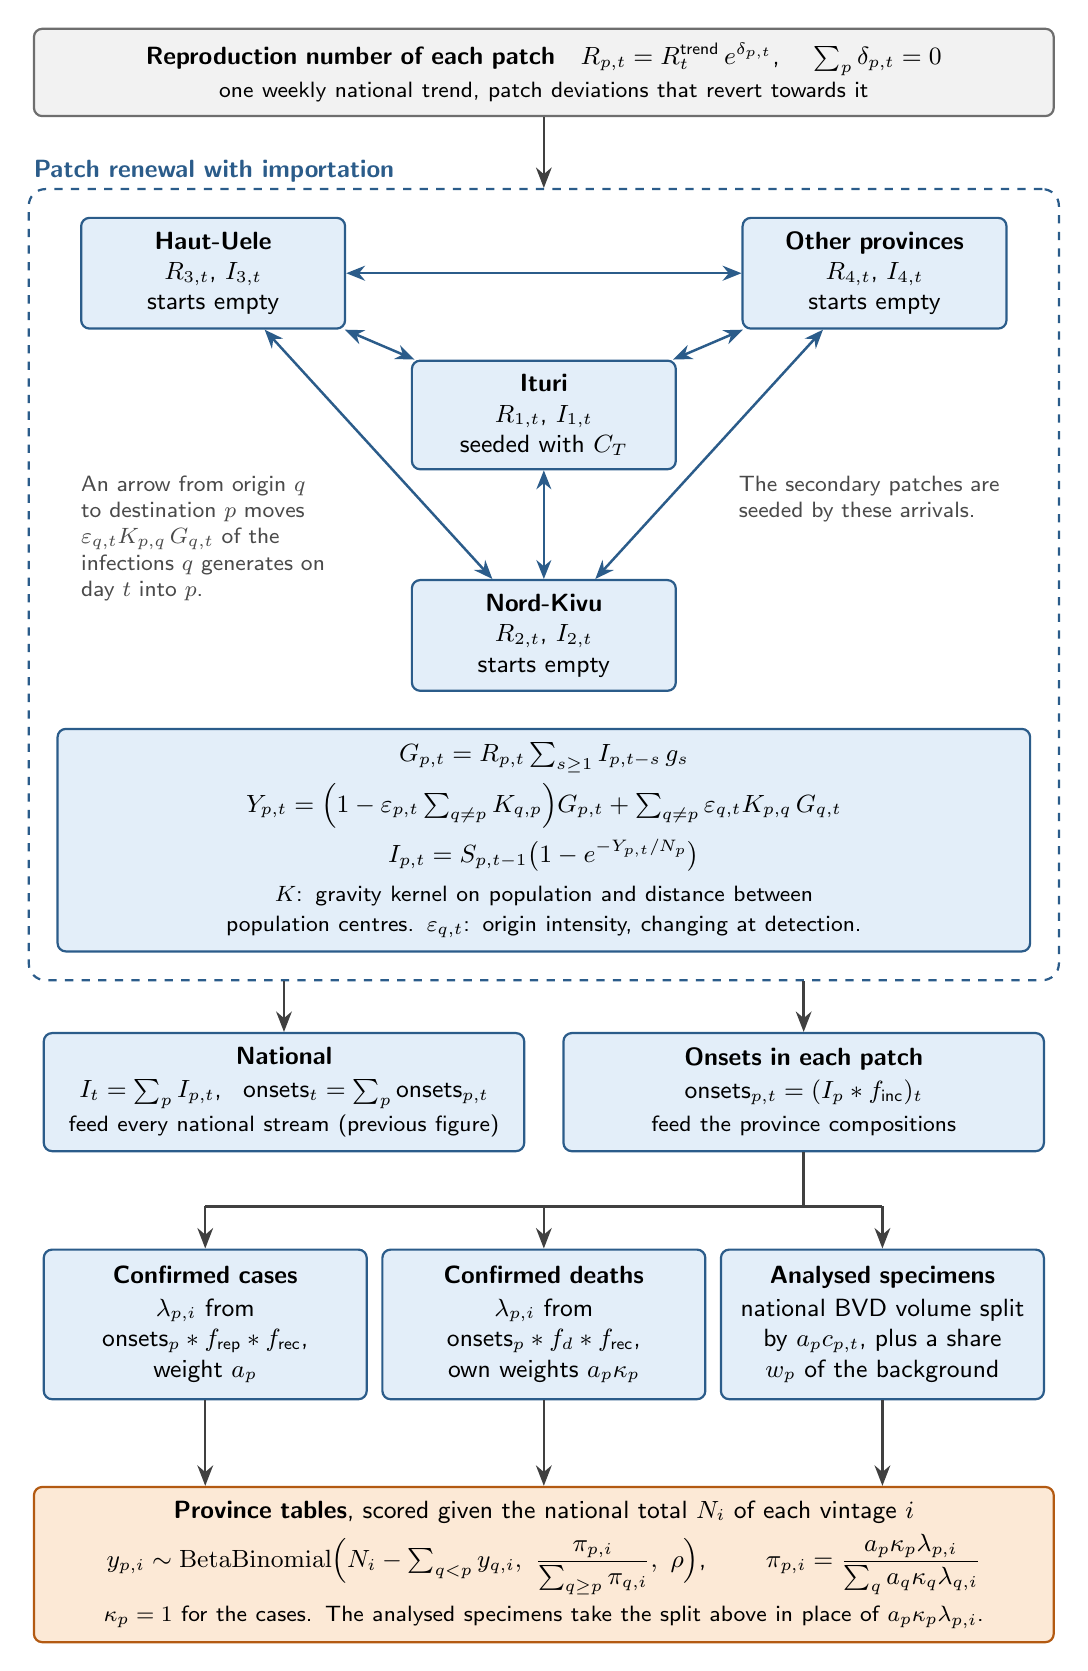
\begin{tikzpicture}[x=1cm,y=1cm]

% ---- Reproduction numbers --------------------------------------------------
\node[param, text width=12.6cm] (rt) at (0,0)
  {\textbf{Reproduction number of each patch}\quad
   $R_{p,t} = R^{\text{trend}}_t\, e^{\delta_{p,t}}$, \quad $\sum_p \delta_{p,t} = 0$\\[1pt]
   {\footnotesize one weekly national trend, patch deviations that revert towards it}};

% ---- Patches ---------------------------------------------------------------
\def\pw{3.0cm}
\node[latent, text width=\pw] (it) at (0,-4.35)
  {\textbf{Ituri}\\ $R_{1,t}$, $I_{1,t}$\\ seeded with $C_T$};
\node[latent, text width=\pw] (hu) at (-4.2,-2.55)
  {\textbf{Haut-Uele}\\ $R_{3,t}$, $I_{3,t}$\\ starts empty};
\node[latent, text width=\pw] (op) at (4.2,-2.55)
  {\textbf{Other provinces}\\ $R_{4,t}$, $I_{4,t}$\\ starts empty};
\node[latent, text width=\pw] (nk) at (0,-7.15)
  {\textbf{Nord-Kivu}\\ $R_{2,t}$, $I_{2,t}$\\ starts empty};

\draw[biflow] (hu) -- (op);
\draw[biflow] (hu) -- (nk);
\draw[biflow] (op) -- (nk);
\draw[biflow] (it) -- (hu);
\draw[biflow] (it) -- (op);
\draw[biflow] (it) -- (nk);

\node[note, text width=3.4cm, anchor=north west] at (-6.0,-5.0)
  {An arrow from origin $q$ to destination $p$ moves
   $\varepsilon_{q,t} K_{p,q}\, G_{q,t}$ of the infections $q$ generates
   on day $t$ into $p$.};
\node[note, text width=3.4cm, anchor=north east] at (6.0,-5.0)
  {The secondary patches are seeded by these arrivals.};

\node[latent, text width=12.0cm] (imp) at (0,-9.75)
  {$G_{p,t} = R_{p,t} \sum_{s \ge 1} I_{p,t-s}\, g_s$\\[3pt]
   $Y_{p,t} = \Bigl(1 - \varepsilon_{p,t} \sum_{q \ne p} K_{q,p}\Bigr) G_{p,t}
    + \sum_{q \ne p} \varepsilon_{q,t} K_{p,q}\, G_{q,t}$\\[3pt]
   $I_{p,t} = S_{p,t-1}\bigl(1 - e^{-Y_{p,t}/N_p}\bigr)$\\[3pt]
   {\footnotesize $K$: gravity kernel on population and distance between
   population centres. $\varepsilon_{q,t}$: origin intensity, changing at detection.}};

\begin{scope}[on background layer]
  \node[group=latentline, fit=(hu) (op) (nk) (imp), inner sep=10pt] (grp) {};
\end{scope}
\node[grouplabel=latentline] at (grp.north west) {Patch renewal with importation};
\draw[flow] (rt.south) -- (rt.south |- grp.north);

% ---- National sum and patch onsets ----------------------------------------
\node[latent, text width=5.75cm, minimum height=15mm] (nat) at (-3.3,-12.95)
  {\textbf{National}\\[1pt] $I_t = \sum_p I_{p,t}$, \enspace
   $\text{onsets}_t = \sum_p \text{onsets}_{p,t}$\\[1pt]
   {\footnotesize feed every national stream (previous figure)}};
\node[latent, text width=5.75cm, minimum height=15mm] (pon) at (3.3,-12.95)
  {\textbf{Onsets in each patch}\\[1pt]
   $\text{onsets}_{p,t} = (I_p * f_{\text{inc}})_t$\\[1pt]
   {\footnotesize feed the province compositions}};
\draw[flow] (-3.3,0 |- grp.south) -- (nat.north);
\draw[flow] (3.3,0 |- grp.south) -- (pon.north);

% ---- Province compositions -------------------------------------------------
\def\cw{3.75cm}
\node[latent, text width=\cw, minimum height=19mm] (pc) at (-4.3,-15.9)
  {\textbf{Confirmed cases}\\[1pt]
   $\lambda_{p,i}$ from\\ $\text{onsets}_{p} * f_{\text{rep}} * f_{\text{rec}}$,\\
   weight $a_p$};
\node[latent, text width=\cw, minimum height=19mm] (pd) at (0,-15.9)
  {\textbf{Confirmed deaths}\\[1pt]
   $\lambda_{p,i}$ from\\ $\text{onsets}_{p} * f_{d} * f_{\text{rec}}$,\\
   own weights $a_p \kappa_p$};
\node[latent, text width=\cw, minimum height=19mm] (pl) at (4.3,-15.9)
  {\textbf{Analysed specimens}\\[1pt]
   national BVD volume split\\ by $a_p c_{p,t}$, plus a share\\
   $w_p$ of the background};

\coordinate (pbus) at (0,-14.4);
\draw[line width=0.9pt, draw=black!75] (-4.3,0 |- pbus) -- (4.3,0 |- pbus);
\draw[line width=0.9pt, draw=black!75] (pon.south) -- (pon.south |- pbus);
\foreach \n in {pc,pd,pl}
  \draw[flow] (\n.north |- pbus) -- (\n.north);

\node[data, text width=12.6cm] (comp) at (0,-18.95)
  {\textbf{Province tables}, scored given the national total $N_i$ of each vintage $i$\\[3pt]
   $y_{p,i} \sim \mathrm{BetaBinomial}\Bigl(N_i - \sum_{q < p} y_{q,i},\
     \dfrac{\pi_{p,i}}{\sum_{q \ge p} \pi_{q,i}},\ \rho\Bigr)$, \qquad
   $\pi_{p,i} = \dfrac{a_p \kappa_p \lambda_{p,i}}{\sum_q a_q \kappa_q \lambda_{q,i}}$\\[3pt]
   {\footnotesize $\kappa_p = 1$ for the cases. The analysed specimens take the split above
   in place of $a_p \kappa_p \lambda_{p,i}$.}};
\foreach \n in {pc,pd,pl}
  \draw[flow] (\n.south) -- (\n.south |- comp.north);

\end{tikzpicture}
\end{document}
